%% This is file `elsarticle-template-1-num.tex',
%%
%% Copyright 2009 Elsevier Ltd
%%
%% This file is part of the 'Elsarticle Bundle'.
%% ---------------------------------------------
%%
%% It may be distributed under the conditions of the LaTeX Project Public
%% License, either version 1.2 of this license or (at your option) any
%% later version.  The latest version of this license is in
%%    http://www.latex-project.org/lppl.txt
%% and version 1.2 or later is part of all distributions of LaTeX
%% version 1999/12/01 or later.
%%
%% Template article for Elsevier's document class `elsarticle'
%% with numbered style bibliographic references
%%
%% $Id: elsarticle-template-1-num.tex 149 2009-10-08 05:01:15Z rishi $
%% $URL: http://lenova.river-valley.com/svn/elsbst/trunk/elsarticle-template-1-num.tex $
%%
\documentclass[final,12pt,a4paper]{elsarticle}

%% Use the option review to obtain double line spacing
%% \documentclass[preprint,review,12pt]{elsarticle}

%% Use the options 1p,twocolumn; 3p; 3p,twocolumn; 5p; or 5p,twocolumn
%% for a journal layout:
%% \documentclass[final,1p,times]{elsarticle}
%% \documentclass[final,1p,times,twocolumn]{elsarticle}
%% \documentclass[final,3p,times]{elsarticle}
%% \documentclass[final,3p,times,twocolumn]{elsarticle}
%% \documentclass[final,5p,times]{elsarticle}
%% \documentclass[final,5p,times,twocolumn]{elsarticle}

%% The graphicx package provides the includegraphics command.
\usepackage{graphicx}
%% The amssymb package provides various useful mathematical symbols
\usepackage{amssymb}
%% The amsthm package provides extended theorem environments
%% \usepackage{amsthm}

\usepackage{booktabs}
\usepackage{xcolor}
\usepackage{sourcecodepro}
\usepackage{url}
\usepackage{listings}
\usepackage[utf8]{inputenc}
\usepackage[brazilian]{babel}
\usepackage{multirow}
\usepackage{textcomp}
\usepackage{caption}
\usepackage[export]{adjustbox}
\usepackage{subcaption}
\usepackage{hyperref}


\definecolor{Accent}{HTML}{157FFF}

\lstdefinestyle{customMtheme}{%
  backgroundcolor={},
  basicstyle=\ttfamily\scriptsize,
  breakatwhitespace=true,
  breaklines=true,
  captionpos=n,
  commentstyle=\color{orange},
  escapeinside={\%*}{*)},
  extendedchars=true,
  frame=n,
  keywordstyle=\color{Accent},
  language=C++,
  rulecolor=\color{black},
  showspaces=false,
  showstringspaces=false,
  xleftmargin=.5cm,
  xrightmargin=.5cm,
  showtabs=false,
  stepnumber=2,
  stringstyle=\color{gray},
  tabsize=4,
  keywords={void, int, float, main,
  if, else, malloc, NULL,
  fprintf, stderr, for, make, gcc, o, Enter, Ctrl},
  otherkeywords={\#pragma, \#include, \&, \*, +, -, /, [, ], >, <, \$, \., std\=c11}
}
\lstset{basicstyle=\ttfamily\scriptsize,style=customMtheme}

\renewcommand*{\UrlFont}{\ttfamily\scriptsize\relax}

\graphicspath{{./img/}}

%% The lineno packages adds line numbers. Start line numbering with
%% \begin{linenumbers}, end it with \end{linenumbers}. Or switch it on
%% for the whole article with \linenumbers after \end{frontmatter}.
%% \usepackage{lineno}

%% natbib.sty is loaded by default. However, natbib options can be
%% provided with \biboptions{...} command. Following options are
%% valid:

%%   round  -  round parentheses are used (default)
%%   square -  square brackets are used   [option]
%%   curly  -  curly braces are used      {option}
%%   angle  -  angle brackets are used    <option>
%%   semicolon  -  multiple citations separated by semi-colon
%%   colon  - same as semicolon, an earlier confusion
%%   comma  -  separated by comma
%%   numbers-  selects numerical citations
%%   super  -  numerical citations as superscripts
%%   sort   -  sorts multiple citations according to order in ref. list
%%   sort&compress   -  like sort, but also compresses numerical citations
%%   compress - compresses without sorting
%%
%% \biboptions{comma,round}

% \biboptions{}

%% Removing lines when no abstract is given
\makeatletter
\renewcommand{\MaketitleBox}{%
    \resetTitleCounters
        \def\baselinestretch{1}%
        \begin{center}
    \def\baselinestretch{1}%
        \Large \@title \par
        \vskip 18pt
        \normalsize\elsauthors \par
        \vskip 10pt
        \footnotesize \itshape \elsaddress \par
        \end{center}
    \vskip 12pt
}
\makeatother

%% Removing custom footer on fist page
\makeatletter
\def\ps@pprintTitle{%
    \let\@oddhead\@empty
        \let\@evenhead\@empty
        \def\@oddfoot{\centerline{\thepage}%
        }%
    \let\@evenfoot\@oddfoot
}%
\makeatother

\journal{MAC 5742-0219 Introdução à Programação Concorrente, Paralela e Distribuída}

\begin{document}

\begin{frontmatter}

%% Title, authors and addresses

\title{EP1: Cálculo do Conjunto de Mandelbrot \\ em Paralelo com Pthreads e OpenMP}

%% use the tnoteref command within \title for footnotes;
%% use the tnotetext command for the associated footnote;
%% use the fnref command within \author or \address for footnotes;
%% use the fntext command for the associated footnote;
%% use the corref command within \author for corresponding author footnotes;
%% use the cortext command for the associated footnote;
%% use the ead command for the email address,
%% and the form \ead[url] for the home page:
%%
%% \title{Title\tnoteref{label1}}
%% \tnotetext[label1]{}
%% \author{Name\corref{cor1}\fnref{label2}}
%% \ead{email address}
%% \ead[url]{home page}
%% \fntext[label2]{}
%% \cortext[cor1]{}
%% \address{Address\fnref{label3}}
%% \fntext[label3]{}


%% use optional labels to link authors explicitly to addresses:
%% \author[label1,label2]{<author name>}
%% \address[label1]{<address>}
%% \address[label2]{<address>}

\author{Felipe Brigalante e Mateus Rocha}

\address{MAC 5742-0219 Introdução à Programação Concorrente, Paralela e Distribuída}

%%\begin{abstract}
%% Text of abstract
%% Suspendisse potenti. Suspendisse quis sem elit, et mattis nisl. Phasellus
%% consequat erat eu velit rhoncus non pharetra neque auctor. Phasellus eu lacus
%% quam. Ut ipsum dolor, euismod aliquam congue sed, lobortis et orci. Mauris eget
%% velit id arcu ultricies auctor in eget dolor. Pellentesque suscipit adipiscing
%% sem, imperdiet laoreet dolor elementum ut. Mauris condimentum est sed velit
%% lacinia placerat. Vestibulum ante ipsum primis in faucibus orci luctus et
%% ultrices posuere cubilia Curae; Nullam diam metus, pharetra vitae euismod sed,
%% placerat ultrices eros. Aliquam tincidunt dapibus venenatis. In interdum tellus
%% nec justo accumsan aliquam. Nulla sit amet massa augue.
%% \end{abstract}
%%
%% \begin{keyword}
%% Science \sep Publication \sep Complicated
%% keywords here, in the form: keyword \sep keyword

%% MSC codes here, in the form: \MSC code \sep code
%% or \MSC[2008] code \sep code (2000 is the default)

%% \end{keyword}

\end{frontmatter}

%%
%% Start line numbering here if you want
%%
%% \linenumbers

%% main text
\section{Apresentação e Análise de Medições para o Programa Sequencial}

\subsection{Detalhes de Implementação}

O programa sequencial foi implementado de duas maneiras, com alocação de memória e I/O e sem. O programa com alocação está igual ao disponibilizado, enquanto no sem alocação e I/O foram retiradas as função e variáveis responsáveis por isso.

\subsection{Resultados}


\begin{figure}[htpb]
\centering
\begin{subfigure}{.55\textwidth}
  \centering
  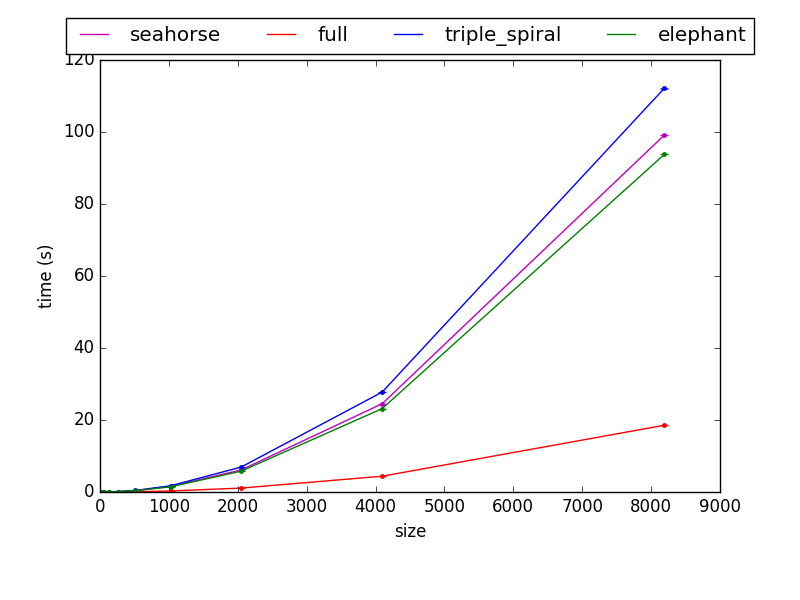
\includegraphics[width=1\linewidth]{image1}
  \caption{Sequencial com alocação}
  \label{fig:image1}
\end{subfigure}%
\begin{subfigure}{.55\textwidth}
  \centering
  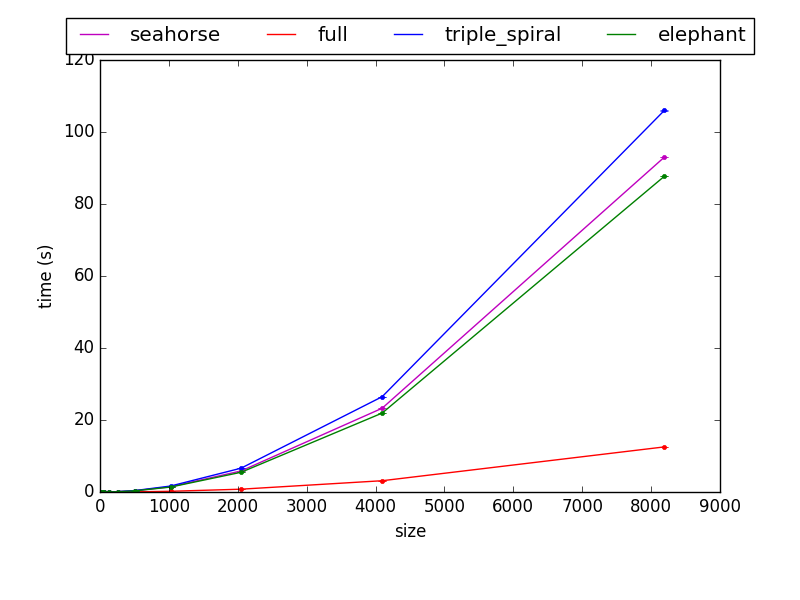
\includegraphics[width=1\linewidth]{image2}
  \caption{Sequencial sem alocação}
  \label{fig:image2}
\end{subfigure}
\caption{1 Thread}
\label{fig:sequencial}
\end{figure}

Em ambas implementações, a região "full" é calculada consideravelmente mais rápido que as outras e isso se deve ao fato de que possivelmente os pontos considerados nessa região demoram menos para convergir. Por isso, tanto no programa com e sem alocação, a proporção de tempo entre as regiões são parecidas.

\clearpage
\begin{figure}[htpb]
    \centering
    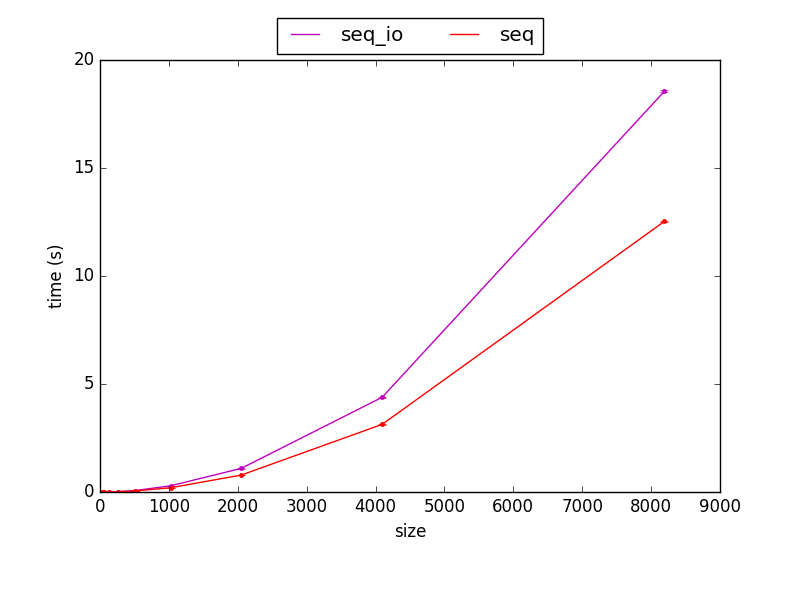
\includegraphics[width=.9\textwidth]{image3}
    \caption{Thread: 1; Região: "full"}
    \label{fig:image3}
\end{figure}

Podemos verificar que as operações de I/O e de alocação de memória aumentam consideravelmente o tempo de execução do programa, em especial em entradas com tamanho grande.

\section{Apresentação e Análise de Medições para o Programa em Pthreads}

\subsection{Detalhes de Implementação}

Para implementar a versão com pthreads foi paralelizado o método \textit{compute\_mandelbrot}. Primeiramente transformamos o \textit{for} duplo em um único \textit{for} para facilitar a paralelização do programa. Foram criadas várias threads que calculam um intervalo de pontos (dependendo do tamanho do chunk) e após terminarem verificam qual o próximo intervalo de pontos a ser calculado. Para isso utilizamos uma variável compartilhada que indica qual o próximo intervalo que deve ser calculado. Naturalmente essa variável tem acesso controlado por meio de um mutex.

O tamanho do chunk utilizado foi 8, e essa escolha foi por duas razões: 
\begin{enumerate}
\item 
A quantidade de pixels sempre vai ser múltipla de 8, Então toda vez que uma thread for processar um chunk, o tempo de execução vai ser parecido (claro que o tempo também vai depender de quanto tempo demora para cada ponto convergir)
\item
Com um chunk de tamanho 8, sempre haverão pelo menos 32 chunks para serem processados. Então no pior dos casos, ou seja, uma imagem 16x16 executando com 32 threads, é esperado que cada thread pelo menos processe um dos chunks.
\end{enumerate}

\subsection{Resultados}

\begin{figure}[htpb]
    \centering
    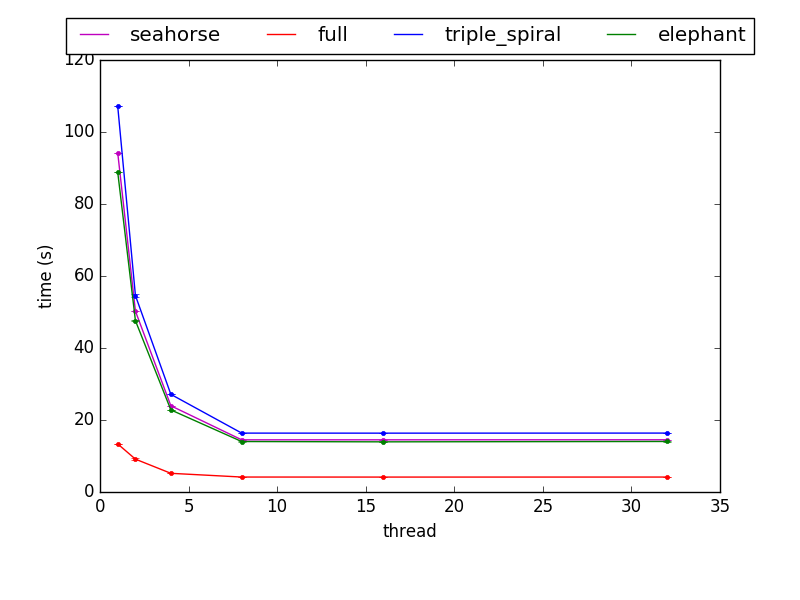
\includegraphics[width=.9\textwidth]{image4}
    \caption{Tamanho: 8192; Método: pthread}
    \label{fig:image4}
\end{figure}

Pode-se notar que nos experimentos com o tamanho da entrada grande, o tempo gasto para execução do programa é inversamente proporcional ao número de threads até que esse se equipare ao número de cores da máquina, nesse caso 8. Depois disso, podemos notar que o tempo gasto permanece praticamente constante, pois somente 8 threads podem rodar paralelamente, isto é, não há ganho de desempenho.

\clearpage
\begin{figure}[htpb]
    \centering
    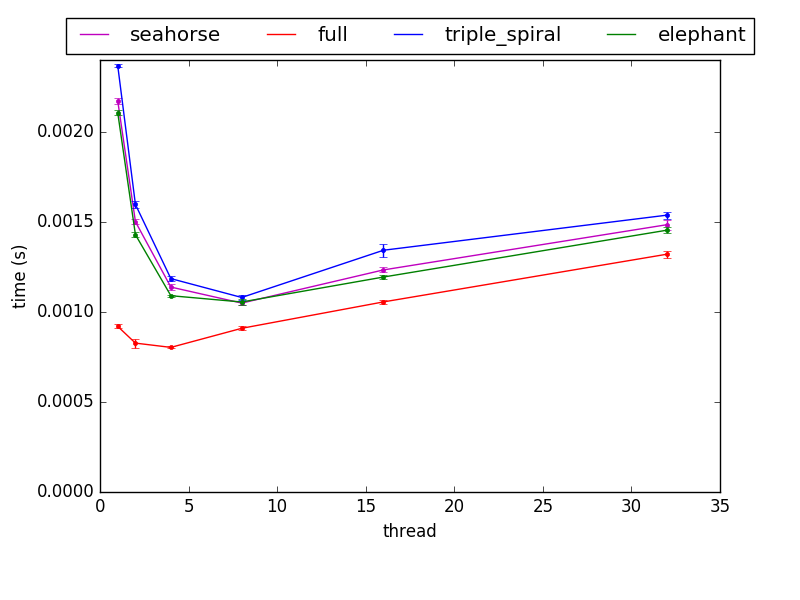
\includegraphics[width=.9\textwidth]{image5}
    \caption{Tamanho: 32; Método: pthread}
    \label{fig:image5}
\end{figure} 

Por outro lado, quando há muitas threads e a entrada do programa é pequena, podemos verificar que o tempo gasto para alocar/organizar as threads acaba interferindo substancialmente no tempo de execução do programa deixando-o algumas vezes até mais lento do que se tivesse menos threads.

\section{Apresentação e Análise de Medições para o Programa em OpenMP}

\subsection{Detalhes de Implementação}

Assim como na implementação usando Pthreads, transformamos o \textit{for} duplo num único \textit{for} e colocamos o pragma adequado do OpenMp para que esse for fosse paralelizado.

\clearpage
\subsection{Resultados}
\begin{figure}[htpb]
\centering
\begin{subfigure}{.55\textwidth}
  \centering
  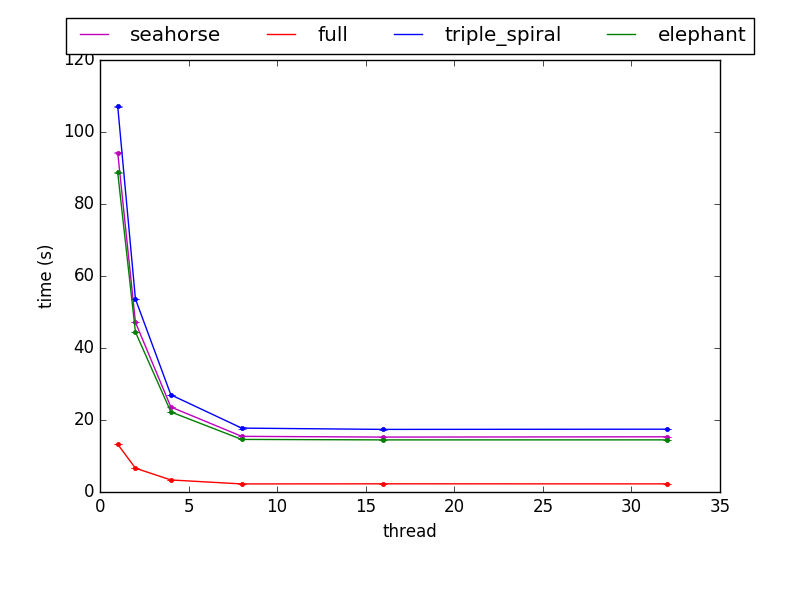
\includegraphics[width=1\linewidth]{image6}
  \caption{Tamanho: 8192}
  \label{fig:image6}
\end{subfigure}%
\begin{subfigure}{.55\textwidth}
  \centering
  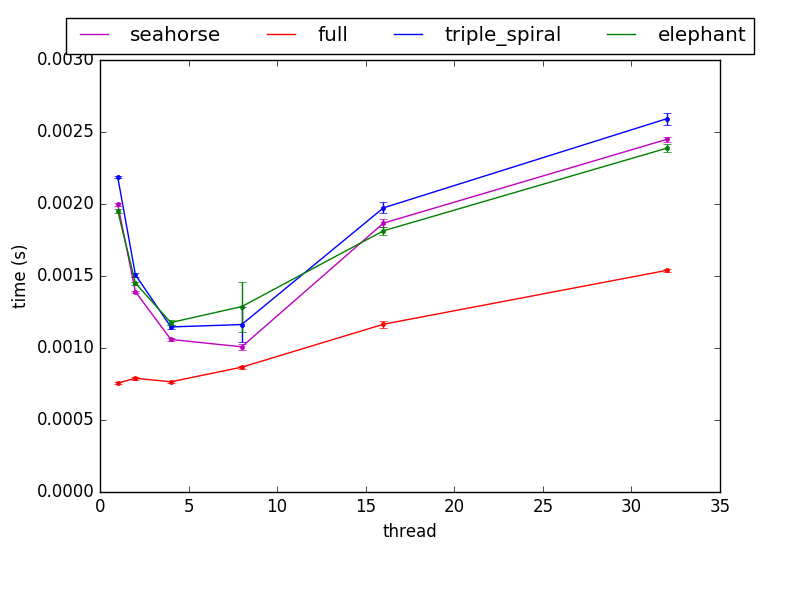
\includegraphics[width=1\linewidth]{image7}
  \caption{Tamanho: 32}
  \label{fig:image7}
\end{subfigure}
\caption{OpenMP}
\label{fig:openmp}
\end{figure}

Os resultados obtidos são semelhantes aos resultados da implementação com Pthreads e as conclusões são as mesmas.

\section{Comparação de Medições entre os Programas}

\begin{figure}[!htpb]
    \centering
    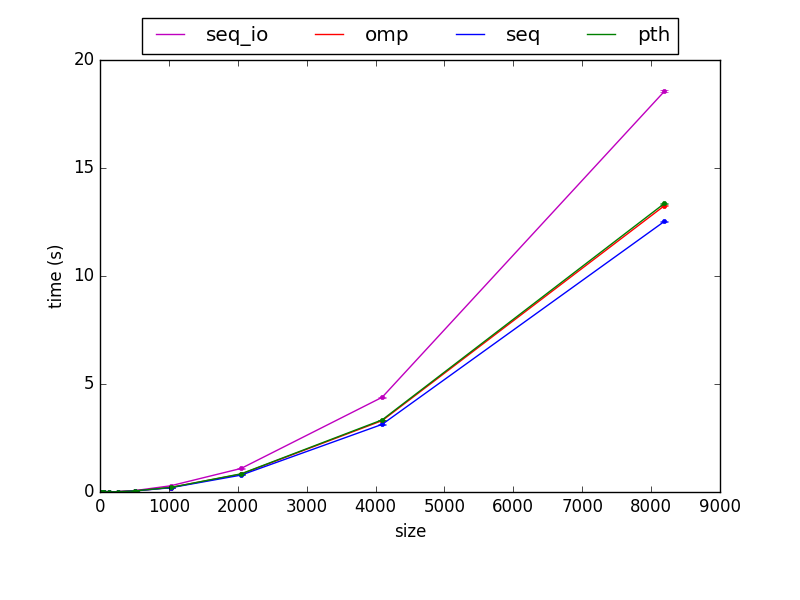
\includegraphics[width=.8\textwidth]{image8}
    \caption{Thread: 1; Região: "full"}
    \label{fig:image8}
\end{figure} 

Podemos perceber que a versão sequencial é mais rápida justamente por não ter nenhuma computação adicional, enquanto as versões paralelas tem que alocar/organizar as threads e a versão sequencial com I/O tem que lidar com a alocação de memória e I/O.

\begin{figure}[htpb]
    \centering
    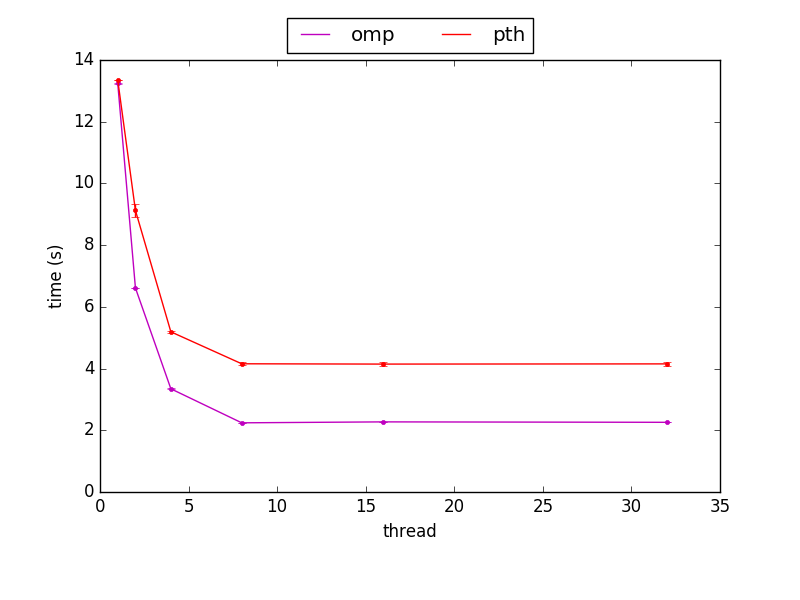
\includegraphics[width=.9\textwidth]{image9}
    \caption{Tamanho: 8192; Região: "full"}
    \label{fig:image9}
\end{figure} 

Em execuções com tamanho de entrada grande vemos que a versão em OpenMP é um pouco mais rápida que a versão em Pthreads, e isso provavelmente se deve ao fato que a versão em OpenMP possui seus códigos mais otimizados do que o os que desenvolvemos na versão em PThreads.

\clearpage
\begin{figure}[htpb]
    \centering
    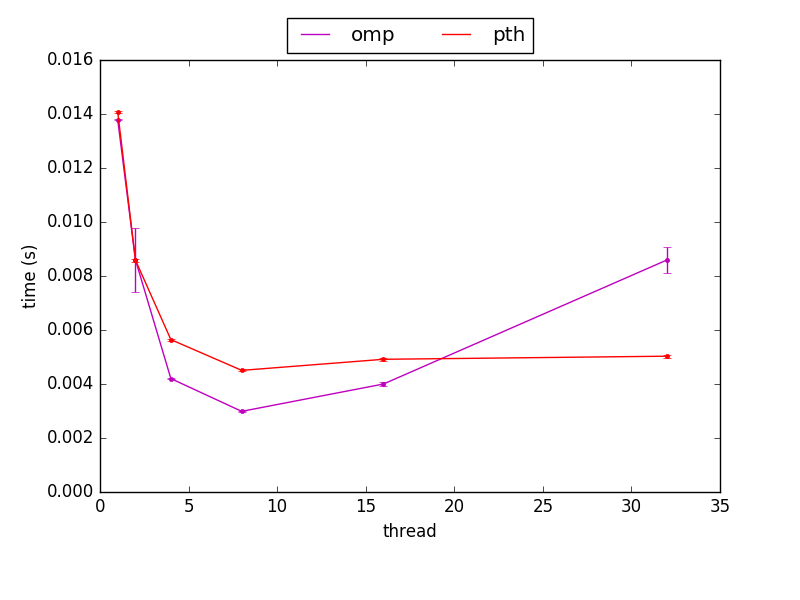
\includegraphics[width=.9\textwidth]{image10}
    \caption{Tamanho: 256; Região: "full"}
    \label{fig:image10}
\end{figure}

Por outro lado em execuções com tamanho de entrada pequena, a versão com Pthreads fica mais rápida e isso acontece pois possivelmente a versão em Pthreads possui um código mais simples do que o código gerado em OpenMP. Pode ser que o OpenMP demore mais na preparação/criação das threads e esse tempo não consegue ser recuperado na execução do algoritmo em si.

\section{Discussão sobre as Medições}

Programas concorrente são dependentes das decisões do escalonador e essas decisões podem variar de acordo com a disponibilidade dos processadores e a troca de contexto. São realizadas várias repetições, pois desse modo é possível identificar o tempo de execução dos programas na maioria dos casos, evitando obter resultados enviesados.

\section{Links}

Todo código feito estará disponível no link abaixo depois do dia de entrega do EP.

\url{https://github.com/mrocha94/MAC5742-0219-EP1}

\end{document}

%%
%% End of file `elsarticle-template-1-num.tex'.
